\section{Results}
\subsection{Figures}
\subsubsection{Mathematical Figures}
Because the primary usecase for \LaTeX\ is the usage in natural sciences and STEM subjects, there are features to display complex mathematical illustrations. 

\begin{figure}
    \caption{Visualization of a normal distribution with the 95\% confidence interval shaded in blue and rejection regions in red.}
    \centering
    \begin{tikzpicture}
        \begin{axis}[
            axis lines=middle,
            enlargelimits=upper,
            domain=-3:3,
            samples=100,
            xtick={-3,-2,-1,0,1,2,3},
            xticklabels={$-3$,$-2$,$-1$,$0$,$1$,$2$,$3$},
            ytick=\empty,
            xlabel={$z$},
            ylabel={Density},
            every axis x label/.style={at={(current axis.right of origin)},anchor=north west},
            every axis y label/.style={at={(current axis.above origin)},anchor=south east}
        ]
        
        % Normal distribution curve
        \addplot[name path=N, domain=-3:3, samples=100, thick] {exp(-x^2/2)/sqrt(2*pi)};
        
        % Confidence interval (shaded region between -1.96 and 1.96)
        \path[name path=lower] (-1.96,0) -- (1.96,0);
        \addplot[blue!30] fill between[of=N and lower, soft clip={domain=-1.96:1.96}];
        
        % Left and right rejection regions
        \path[name path=left] (-3,0) -- (-1.96,0);
        \path[name path=right] (1.96,0) -- (3,0);
        \addplot[red!50, pattern=north east lines, pattern color=red] fill between[of=N and left, soft clip={domain=-3:-1.96}];
        \addplot[red!50, pattern=north east lines, pattern color=red] fill between[of=N and right, soft clip={domain=1.96:3}];
        
        % Vertical dashed lines for z = -1.96 and z = 1.96
        \addplot[dashed] coordinates {(-1.96,0) (-1.96,0.2)};
        \addplot[dashed] coordinates {(1.96,0) (1.96,0.2)};
        
        % Labels
        \node[anchor=north] at (axis cs:-1.96,0) {$-1.96$};
        \node[anchor=north] at (axis cs:1.96,0) {$1.96$};
        \node at (axis cs:0,0.05) {95\% CI};
        
        \end{axis}
    \end{tikzpicture}
    \label{fig:confidence_interval}
\end{figure}
\newpage
\subsubsection{External Figures}
External image files like .png or .jpg images can easily be added and automatically numbered as well. Note that the image file should be in the project folder to refer to it.

\begin{figure}
    %\centering
     \caption{An example figure}
     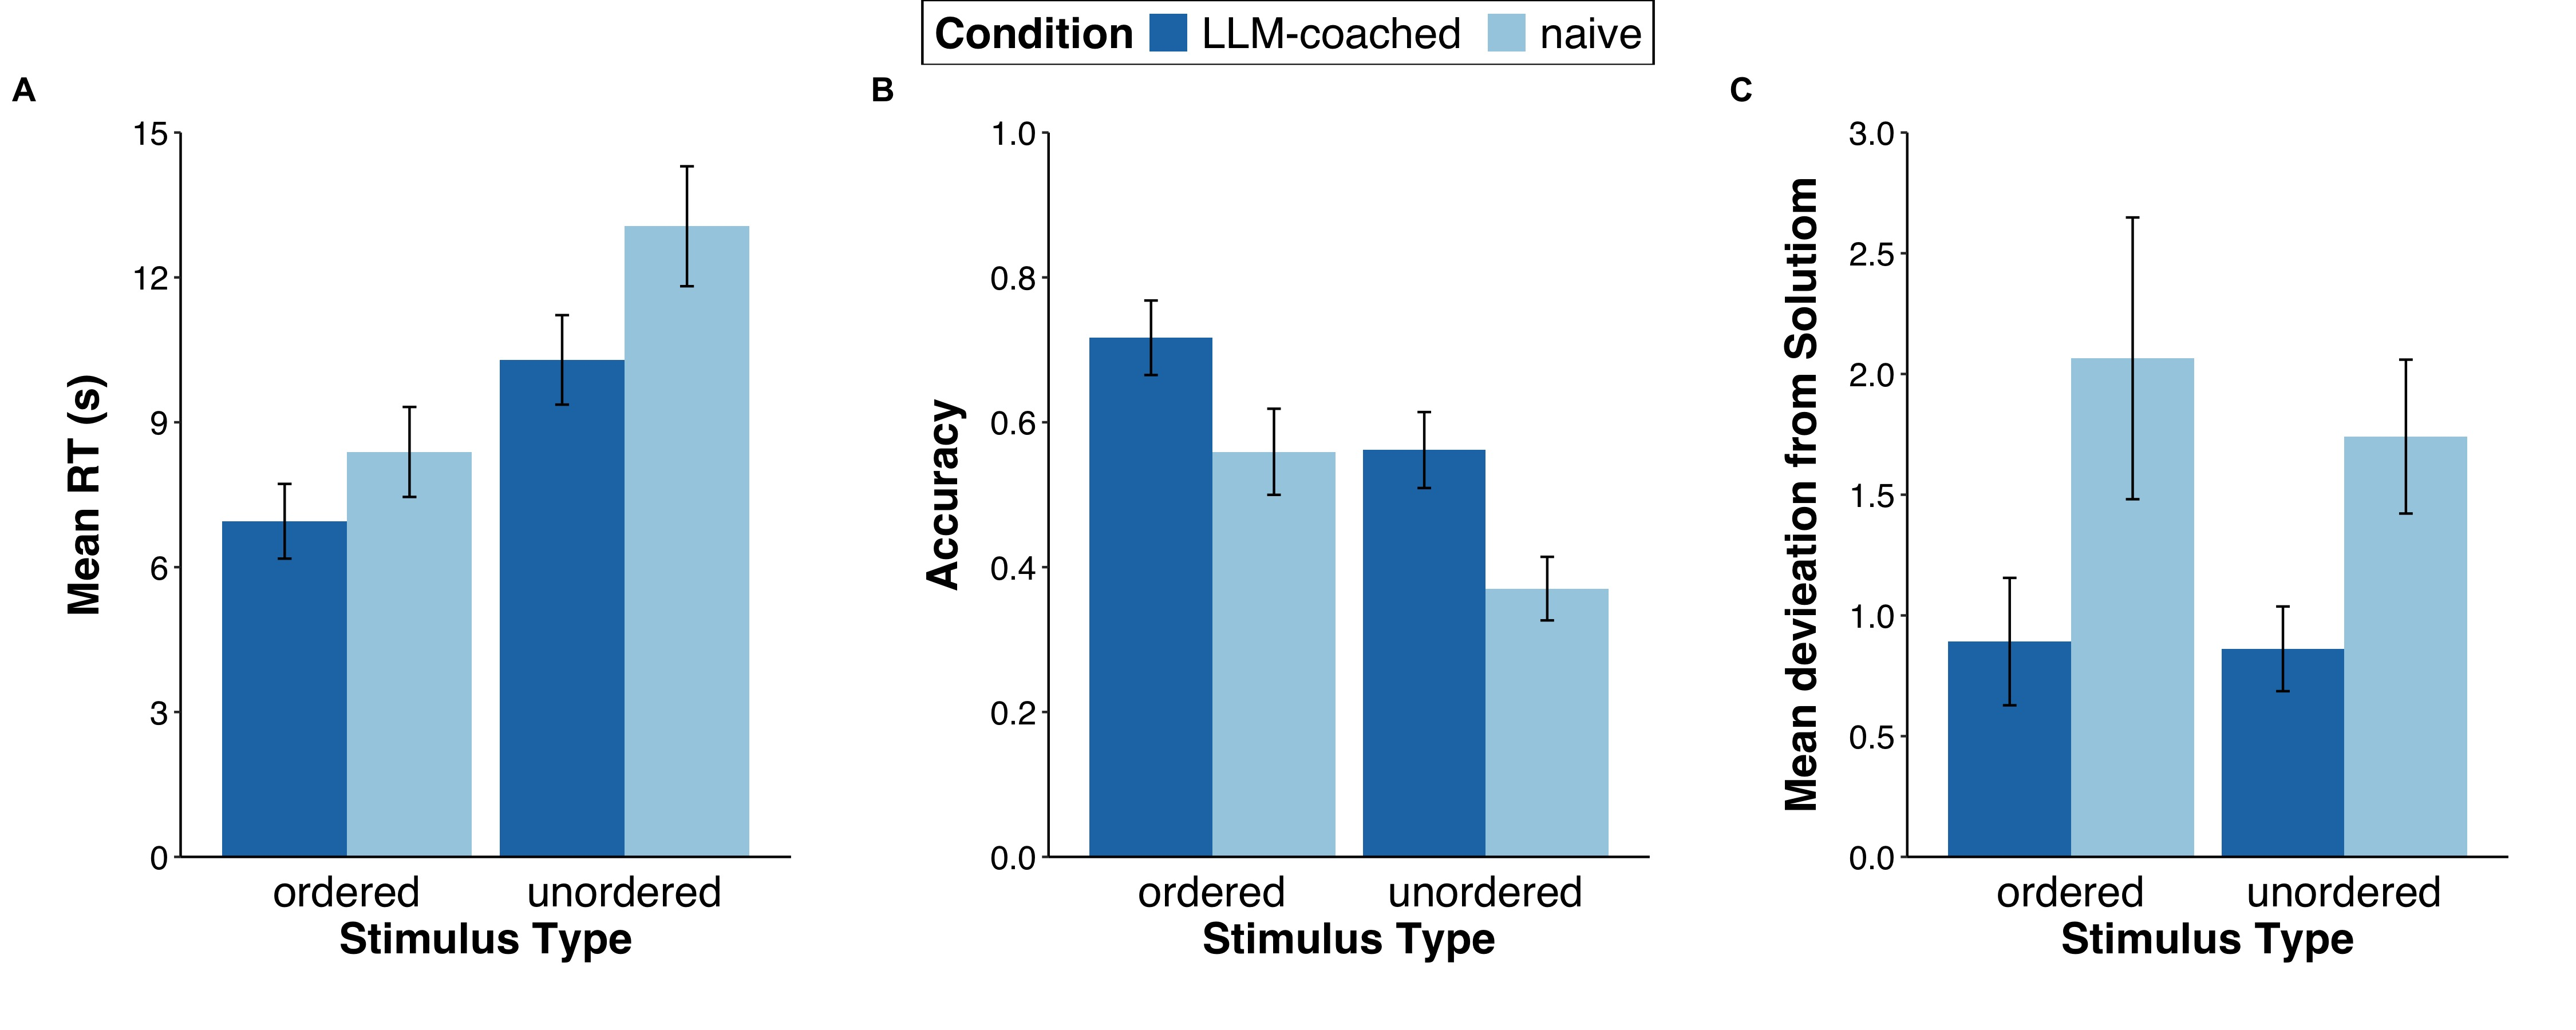
\includegraphics[width=\linewidth]{Tables & Figures/DCTplot.jpg}
     
     %\label{fig:enter-label}
 \end{figure}